%-------------------------------------------------------------------------------
%	PAQUETES Y OTRAS CONFIGURACIONES
%-------------------------------------------------------------------------------
%-------------------------------------------------------------------------------
%	PAQUETES Y OTRAS CONFIGURACIONES
%-------------------------------------------------------------------------------
%\documentclass{tufte-handout}
%\documentclass[paper=letter, landscape, fontsize=16pt]{scrartcl}
\documentclass{beamer}
\usepackage{wrapfig}
\usepackage{geometry}
%\geometry{left=1.2cm, right=1.2cm, top=1.5cm, bottom=3cm}
\usepackage{color}
\usepackage[utf8]{inputenc}
\usepackage[T1]{fontenc}
\usepackage{cmbright}
\usepackage[sfdefault]{noto}
\usepackage[ttdefault=true]{AnonymousPro}
\usepackage[T1]{fontenc}
\normalfont
%\usepackage{graphicx}
\usepackage{multicol}
%\usepackage{circuitikz}
\usepackage{amsmath}
\usepackage{mathtools}

\usepackage[american]{circuitikz}
\usepackage{tikz-timing}
\usetikzlibrary{decorations.pathreplacing}
\usepackage{tikz}
\usepackage[framemethod=tikz]{mdframed}
\usetikzlibrary{arrows, positioning}
\usepackage{tkz-euclide}

%\usepackage{sectsty} % Paquete para configuración de secciones
%\allsectionsfont{\centering \normalfont \scshape} % Los títulos de las secciones son centrados, con la misma fuente y pequeñas mayúsculas

\usetikztiminglibrary{nicetabs}
\usepackage{todonotes}
\usepackage{microtype}
\renewcommand{\figurename}{Figura}

\usepackage{listings}
\renewcommand{\lstlistingname}{Código}
\lstdefinestyle{mystyle}{
    basicstyle=\footnotesize\ttfamily,
    breakatwhitespace=false,
    breaklines=true,
    captionpos=b,
    keepspaces=true,
    numbers=left,
    numbersep=5pt,
    showspaces=false,
    showstringspaces=false,
    showtabs=false,
    tabsize=2
}
\lstset{style=mystyle}

% \usepackage{fancyhdr} % Paquete para personalizar pies y cabeceras de página
% \pagestyle{fancyplain} % Todas las páginas con las mismas cabeceras y pies de página
% \fancyhead{} % Sin cabecera
% \fancyfoot[L]{} % Vacío en la izquierda del pie de página
% \fancyfoot[C]{} % Vacío en el centro del pie de página
% \fancyfoot[R]{\thepage} % Número de página en el pie de pagina
% \renewcommand{\headrulewidth}{0pt} % Sin lineas en la cabecera
% \renewcommand{\footrulewidth}{0pt} % Sin lineas en el pie de página
% \setlength{\headheight}{13.6pt} % Altura de cabecera
%
% \numberwithin{equation}{section} % Numera ecuaciones en cada sección
% \numberwithin{figure}{section} % Numera figuras en cada sección
% \numberwithin{table}{section} % Numera tablas en cada sección
%
% \setlength\parindent{0pt} % Quita la indentación de los párrafos

\newcommand{\horrule}[1]{\rule{\linewidth}{#1}} % Comando personalizado para hacer linea horizontal

\let\oldfootnotesize\footnotesize
\renewcommand*{\footnotesize}{\oldfootnotesize\tiny}
%-------------------------------------------------------------------------------
%	TITULO
%-------------------------------------------------------------------------------
\title{Práctica 4 - Sensores y actuadores}
\author{Roberto Cadena Vega}
\date{}
%-------------------------------------------------------------------------------
%	EMPIEZA EL DOCUMENTO
%-------------------------------------------------------------------------------
\begin{document}
\beamertemplatenavigationsymbolsempty
\maketitle
%-------------------------------------------------------------------------------
%	OBJETIVOS
%-------------------------------------------------------------------------------
\begin{frame}
	\frametitle{Objetivo}
	Utilizar algoritmos de control automático y un sistema de visión artificial para programar comportamientos estables de movimiento en el Robotino FESTO.
\end{frame}
%-------------------------------------------------------------------------------
%	EQUIPO
%-------------------------------------------------------------------------------
\begin{frame}
	\frametitle{Equipo}
	El siguiente equipo será proporcionado por el laboratorio, siempre y cuando lleguen en los primeros 15 minutos de la práctica.
	\begin{itemize}
		\item Plataforma de desarrollo Robotino FESTO
		\item Computadora con el software Robotino View\footnote{https://www.festo-didactic.com/int-en/services/robotino/programming/robotino-view/?fbid=aW50LmVuLjU1Ny4xNy4zNC4xNDI2} y Robotino SIM\footnote{https://www.festo-didactic.com/int-en/services/robotino/simulation/?fbid=aW50LmVuLjU1Ny4xNy4zNC4xNDQy} instalado
	\end{itemize}
\end{frame}
%-------------------------------------------------------------------------------
%	CONOCIMIENTOS PREVIOS
%-------------------------------------------------------------------------------
\begin{frame}
	\frametitle{Conocimientos Previos}
\end{frame}

\begin{frame}
	\frametitle{Introducción}
	En la práctica anterior programamos un algoritmo de control automático para controlar la posición del Robotino relativa a un objeto cercano, por medio de los sensores infrarojos de distancia.

	Sin embargo este algoritmo desarrollaba solo una función, si queremos programar comportamientos complejos en el Robotino necesitamos aprender la capacidad de ejecutar diagramas de tipo GRAFCET; lo que nos permitirá ejecutar diferentes programas en diferentes condiciones.
\end{frame}

\begin{frame}
	\frametitle{Control secuencial}
		Hasta el momento hemos utilizado solo la pestaña que esta marcada como Step 1, para diseñar el diagrama tipo GRAFCET con la secuencia de pasos a ejecutar tenemos que entrar en la pestaña de Programa Principal (Main).

		\begin{figure}
			\begin{center}
				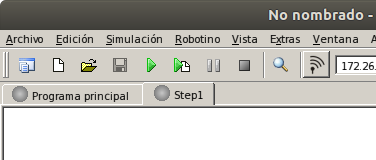
\includegraphics[width=0.9\textwidth]{images/00-control-multiple/00.png}
				\label{fig:multiple-00}
			\end{center}
		\end{figure}
\end{frame}

\begin{frame}
	\begin{columns}
		\column{0.4\textwidth}
		\begin{figure}
			\begin{center}
				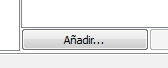
\includegraphics[width=0.9\textwidth]{images/00-control-multiple/03-01.png}
				\label{fig:multiple-03-01}
			\end{center}
		\end{figure}
		\begin{figure}
			\begin{center}
				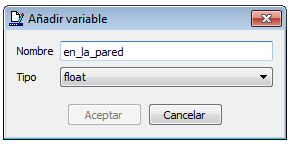
\includegraphics[width=0.9\textwidth]{images/00-control-multiple/04.png}
				\label{fig:multiple-04}
			\end{center}
		\end{figure}
		\begin{figure}
			\begin{center}
				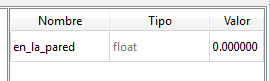
\includegraphics[width=0.9\textwidth]{images/00-control-multiple/03-02.png}
				\label{fig:multiple-03-02}
			\end{center}
		\end{figure}

		\column{0.6\textwidth}
		El primer paso es definir una variable, la cual utilizaremos para determinar en que momento debemos cambiar de un programa a otro; en este caso se llamará \texttt{en\_la\_pared}, será de tipo flotante y tendrá un valor de 0.
	\end{columns}
\end{frame}

\begin{frame}
	\begin{columns}
		\column{0.6\textwidth}
		Una vez que tenemos nuestra variable, podemos hacer nuestro diagrama de GRAFCET el cual, en un principio, tiene solo el programa Step1 y agregaremos nosotros el programa Step2 con el boton de agregar bloque abajo estando seleccionado el primer programa. Ademas modificaremos la condición necesaria para cambiar del primer programa al segundo, colocando el nombre de la variable que definimos.

		\column{0.4\textwidth}
		\begin{figure}
			\begin{center}
				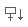
\includegraphics[width=0.4\textwidth]{images/00-control-multiple/03-03.png}
				\label{fig:multiple-03-03}
			\end{center}
		\end{figure}
		\begin{figure}
			\begin{center}
				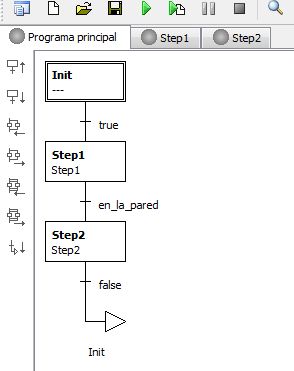
\includegraphics[width=0.9\textwidth]{images/00-control-multiple/03-04.png}
				\label{fig:multiple-03-04}
			\end{center}
		\end{figure}
	\end{columns}
\end{frame}

\begin{frame}
	\begin{columns}
		\column{0.5\textwidth}
		\begin{figure}
			\begin{center}
				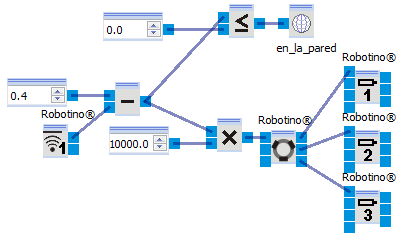
\includegraphics[width=0.95\textwidth]{images/00-control-multiple/01.png}
				\label{fig:multiple-01}
			\end{center}
		\end{figure}

		\column{0.5\textwidth}
		Ahora tenemos que programar los algoritmos de control de cada paso, empezando en el programa Step1, el cual es muy similar al de la práctica 3, pero agregamos una comparación para saber cuando el Robotino ya ha llegado a la pared, lo cual hará que la variable \texttt{en\_la\_pared} tenga un valor \texttt{verdadero} cuando el Robotino llegue a la pared.
	\end{columns}
\end{frame}

\begin{frame}
	\begin{columns}
		\column{0.5\textwidth}
		Y en el programa 2 ponemos el mismo comportamiento para el movimiento hacia adelante y hacia atras, pero agregamos un algoritmo de control para el movimiento rotacional sobre el eje del Robotino; recordando que los sensores 2 y 3 estan al frente y a la izquierda del Robotino y los sensores 8 y 9 estan al frente y a la derecha del Robotino, la operación que estamos realizando se reduce a

		\begin{equation*}
			\dot{\theta} = (S_2 + S_3 - S_8 - S_9)\cdot 100
		\end{equation*}

		\column{0.5\textwidth}
		\begin{figure}
			\begin{center}
				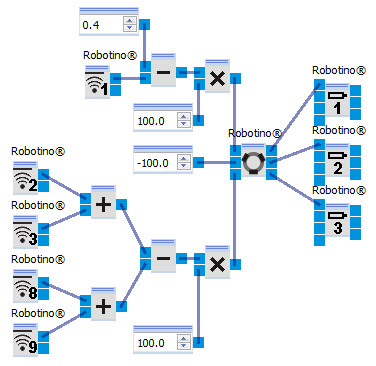
\includegraphics[width=0.95\textwidth]{images/00-control-multiple/02.png}
				\label{fig:multiple-02}
			\end{center}
		\end{figure}
	\end{columns}
\end{frame}

\begin{frame}
	\begin{columns}
		\column{0.5\textwidth}
		El movimiento lateral simplemente se mueve en una dirección todo el tiempo, de tal manera que el comportamiento final será que el Robotino tratará de seguir la pared a una distancia definida, girando cuando se encuentre algún obstaculo. En este punto, deberás guardar tu programa y validarlo con la plataforma Robotino en la vida real.

		\column{0.5\textwidth}
		\begin{figure}
			\begin{center}
				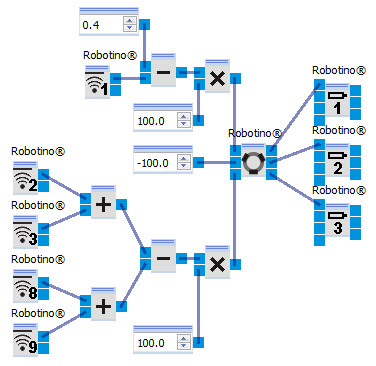
\includegraphics[width=0.95\textwidth]{images/00-control-multiple/02.png}
			\end{center}
		\end{figure}
	\end{columns}
\end{frame}

\begin{frame}
	\frametitle{Visión artificial}
	\begin{columns}
		\column{0.4\textwidth}
		\begin{figure}
			\begin{center}
				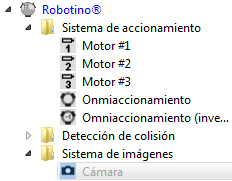
\includegraphics[width=0.8\textwidth]{images/01-vision-artificial/01-01.png}
				\label{fig:vision-01-01}
			\end{center}
		\end{figure}
		\begin{figure}
			\begin{center}
				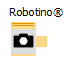
\includegraphics[width=0.4\textwidth]{images/01-vision-artificial/01-02.png}
				\label{fig:vision-01-02}
			\end{center}
		\end{figure}

		\column{0.6\textwidth}
		Ya que entendemos como crear comportamientos complejos para nuestro Robotino el siguiente paso es agregar un nuevo sensor a nuestro arsenal de automatización; en un programa completamente nuevo agrega el elemento Camara que se encuentra en Sistema de imagenes.
	\end{columns}
\end{frame}

\begin{frame}
	\begin{columns}
		\column{0.5\textwidth}
		Si corremos este programa con solo la camara en el, y hacemos doble clic en el icono de la función, podremos tener una ventana con las imagenes de la camara frontal del Robotino.

		\column{0.5\textwidth}
		\begin{figure}
			\begin{center}
				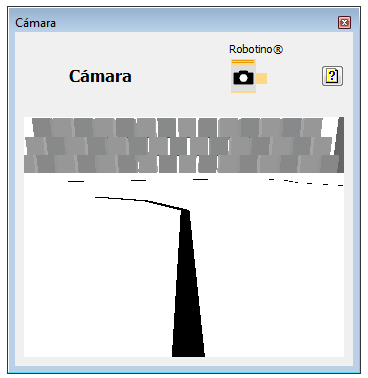
\includegraphics[width=0.95\textwidth]{images/01-vision-artificial/02.png}
			\end{center}
		\end{figure}
	\end{columns}
\end{frame}

\begin{frame}
	\begin{columns}
		\column{0.6\textwidth}
		\begin{figure}
			\begin{center}
				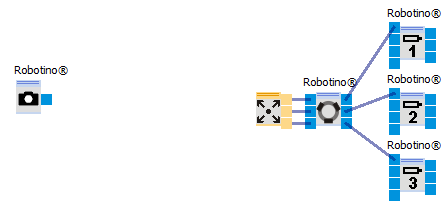
\includegraphics[width=0.95\textwidth]{images/01-vision-artificial/03.png}
			\end{center}
		\end{figure}
		\begin{figure}
			\begin{center}
				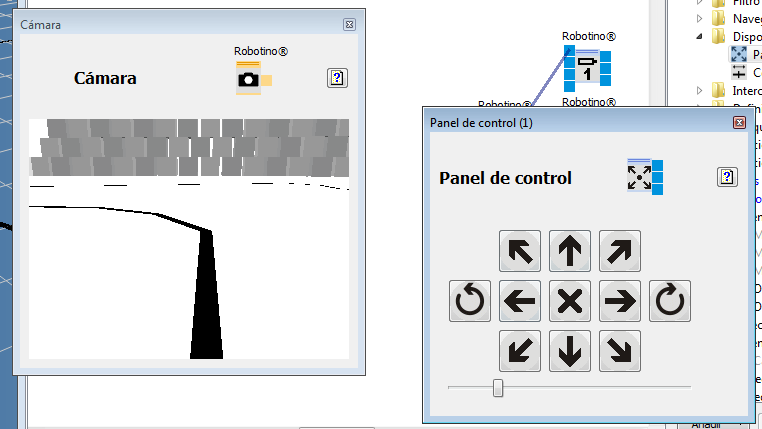
\includegraphics[width=0.95\textwidth]{images/01-vision-artificial/04.png}
			\end{center}
		\end{figure}

		\column{0.4\textwidth}
		O bien, si agregamos el control de motores a nuestro programa, podremos manipular el Robotino mientras vemos las imagenes de su camara frontal
	\end{columns}
\end{frame}

\begin{frame}
	\begin{columns}
		\column{0.6\textwidth}
		Pero las imagenes de la camara por si solas no son suficientes para manipular el comportamiento de nuestro Robotino, tenemos que hacer un procesamiento de los datos para obtener información relevante, por ejemplo, para encontrar objetos con un cierto color en nuestro ambiente. Ahora agregaremos la función de Busqueda de gamas de colores, que se encuentra en Procesamiento de imágenes.

		\column{0.4\textwidth}
		\begin{figure}
			\begin{center}
				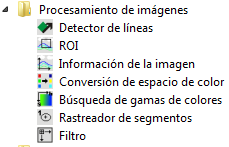
\includegraphics[width=0.9\textwidth]{images/01-vision-artificial/05-01.png}
			\end{center}
		\end{figure}
		\begin{figure}
			\begin{center}
				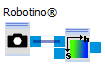
\includegraphics[width=0.5\textwidth]{images/01-vision-artificial/05-02.png}
			\end{center}
		\end{figure}
	\end{columns}
\end{frame}

\begin{frame}
	\begin{columns}
		\column{0.6\textwidth}
		\begin{figure}
			\begin{center}
				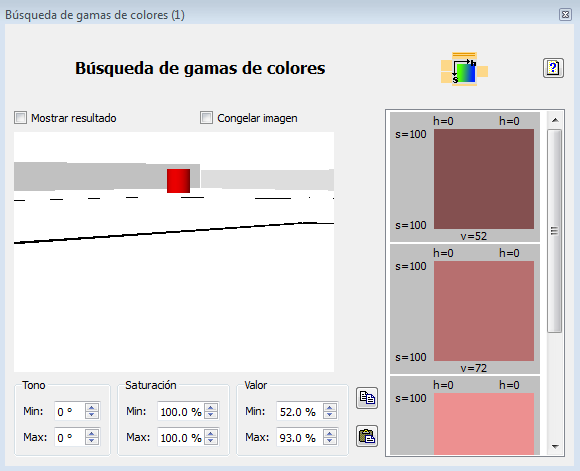
\includegraphics[width=0.7\textwidth]{images/01-vision-artificial/07.png}
			\end{center}
		\end{figure}
		\begin{figure}
			\begin{center}
				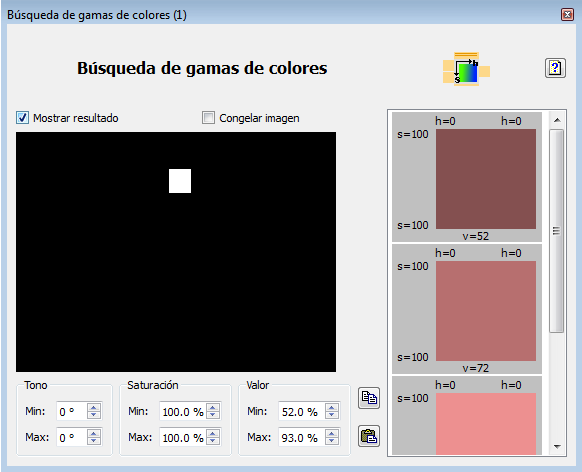
\includegraphics[width=0.7\textwidth]{images/01-vision-artificial/08.png}
			\end{center}
		\end{figure}

		\column{0.4\textwidth}
		Si abrimos la función recien insertada, tendremos una ventana en donde podemos escoger la gama de colores que queremos aislar, una vez seleccionados los colores debemos ver como todo el resto de la imagen se vuelve negra si seleccionamos mostrar resultado.
	\end{columns}
\end{frame}

\begin{frame}
	\begin{columns}
		\column{0.4\textwidth}
		Agregando ahora el Rastreador de segmentos, podremos ver como este nos va dar información importante de las imagenes obtenidas, lo mas importante, la posición en el eje $x$.

		\column{0.6\textwidth}
		\begin{figure}
			\begin{center}
				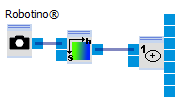
\includegraphics[width=0.5\textwidth]{images/01-vision-artificial/09.png}
			\end{center}
		\end{figure}
		\begin{figure}
			\begin{center}
				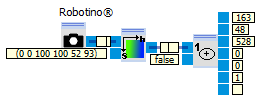
\includegraphics[width=0.7\textwidth]{images/01-vision-artificial/10.png}
			\end{center}
		\end{figure}
		\begin{figure}
			\begin{center}
				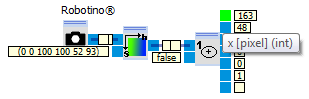
\includegraphics[width=0.7\textwidth]{images/01-vision-artificial/11.png}
			\end{center}
		\end{figure}
	\end{columns}
\end{frame}

\begin{frame}
	\begin{columns}
		\column{0.5\textwidth}
		\begin{figure}
			\begin{center}
				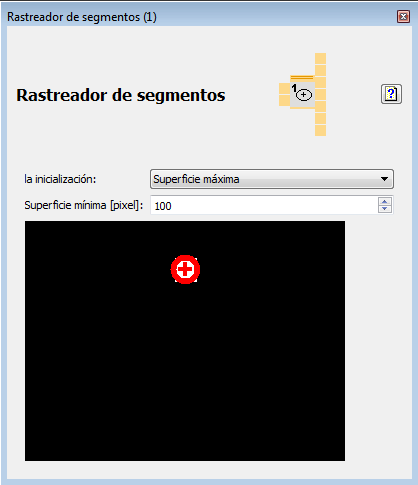
\includegraphics[width=0.9\textwidth]{images/01-vision-artificial/13.png}
			\end{center}
		\end{figure}

		\column{0.5\textwidth}
		Analizando esta información, el valor que obtenemos como primer salida de la función Rastreador de segmentos es la posición del centroide del objeto detectado dentro de la imagen.
	\end{columns}
\end{frame}

\begin{frame}
	\begin{columns}
		\column{0.35\textwidth}
		Si aplicamos un algoritmo de control a este parametro, queriendo que el objeto encontrado este en el centro de la imagen (la imagen tiene 320 pixeles de ancho, por lo que el centro es la posición 160), podremos construir un diagrama como el de al lado.

		\column{0.65\textwidth}
		\begin{figure}
			\begin{center}
				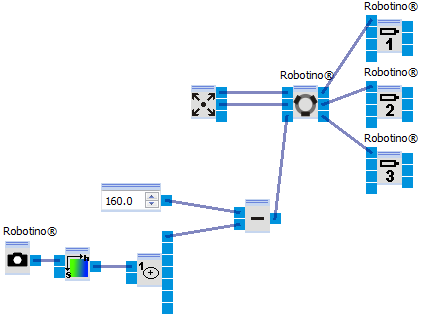
\includegraphics[width=0.95\textwidth]{images/01-vision-artificial/12.png}
			\end{center}
		\end{figure}
	\end{columns}
\end{frame}

\begin{frame}
	\begin{columns}
		\column{0.35\textwidth}
		El resultado de este algoritmo de control es que una vez que el Robotino ha encontrado un objeto con el color que queremos, cuando movamos el Robotino lo hará siempre viendo hacia ese objeto. En este punto, deberás guardar tu programa y validarlo con la plataforma Robotino en la vida real.

		\column{0.65\textwidth}
		\begin{figure}
			\begin{center}
				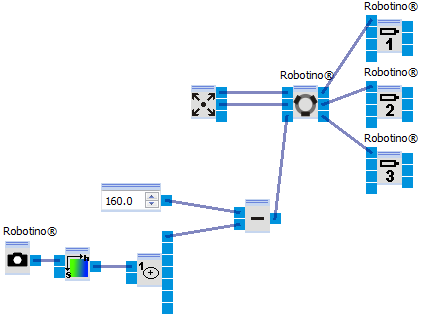
\includegraphics[width=0.95\textwidth]{images/01-vision-artificial/12.png}
			\end{center}
		\end{figure}
	\end{columns}
\end{frame}
%-------------------------------------------------------------------------------
%	DESARROLLO
%-------------------------------------------------------------------------------
\begin{frame}
	\frametitle{Desarrollo}

	\begin{itemize}
		\item Valida los programas requeridos en el area de Conocimientos previos
		\item Diseña un conjunto de programas de tal manera que el Robotino gire sobre su eje hasta encontrar un objeto del color definido por ti y una vez que lo encuentre se mueva hacia el y pare a aproximadamente $30cm$ de el. Valida tu programación en simulación y en la vida real.
	\end{itemize}
\end{frame}
%-------------------------------------------------------------------------------
%	CONCLUSIONES
%-------------------------------------------------------------------------------
\begin{frame}
	\frametitle{Conclusiones}
	El alumno deberá describir sus conclusiones al final de su reporte de práctica.
\end{frame}
%-------------------------------------------------------------------------------
%	FIN DEL DOCUMENTO
%-------------------------------------------------------------------------------
\end{document}
